\section{物联网}

\subsection{物联网简介}

\begin{frame}
    \frametitle{为什么要把物体联到网络}
    \qquad 物联网，就是物物相连的互联网，如把销售人员、货物、快递员、货车、消费者等连起来形成快递物联网。通过把相关的物体和设备都联网，能够随时观测状态，监控运行情况并进行控制和调整……一旦发生故障就能及时发现，给予修理或者更换。比如家中的水表电表和住户以及相关机构联网，就可以通过网络终端查看用水用电情况，及时缴费甚至自动续费等。这样，就可以把现在许多需要人力完成的诸如抄表、巡视、看监控器等工作交给机器来干。

    \qquad 其实，物联网是在帮助人类“偷懒”，把人类从简单的重复性工作中解放出来，去从事更有创造性的工作。以前，我们很难直接观测到机器、物品、设施的很多参数，也不可能去监控。然而，有了物联网之后，这些就都可以被自动观测并传输到控制中心，用计算机来自动判断数据是不是正常。如果不正常，机器就向人类发出警报。
\end{frame}

\begin{frame}
    \frametitle{物联网}
    物联网（The Internet of Things，简称IOT）是指通过传感器等各种装置与技术，实时采集各种需要的信息，通过各类可能的网络接入，实现物与物、物与人的泛在连接，实现对物品和过程的智能化感知、识别和管理。

    \begin{figure}[htpb]
      \centering
      
\includegraphics[height=.35\linewidth]{IOT1} \quad
      
\includegraphics[height=.35\linewidth]{IOT2}
    \end{figure}
\end{frame}

\begin{frame}
    \frametitle{物联网与互联网的不同之处}
    \only<1>{
      \begin{figure}[htpb]
        \centering
        
\includegraphics[width=\linewidth]{物联网VS互联网1}
    \end{figure}
    }
    \only<2>{
      \begin{figure}[htpb]
        \centering
        
\includegraphics[width=\linewidth]{物联网VS互联网2}
    \end{figure}
    }
\end{frame}


\subsection{物联网应用}

\begin{frame}
    \frametitle{智慧农业}
    将物联网技术用于大田种植、设施园艺、畜禽养殖、水产养殖、农产品物流、农副产品食品安全质量监控与溯源等领域，实现对农业生产过程中的土壤、环境、水资源的实时监测，对动植物生长过程的精细管理，对农副产品生产的全过程监控与可追溯管理，对大型农业机械作业服务的优化调度。

    \begin{figure}[htpb]
      \centering
      
\includegraphics[height=.275\linewidth]{智慧农业1}
      
\includegraphics[height=.275\linewidth]{智慧农业}
    \end{figure}
\end{frame}


\begin{frame}
    \frametitle{物联网农业应用案例：智慧温室大棚}
    \begin{figure}[htpb]
        \centering
        
\includegraphics[width=.7\linewidth]{智慧大棚}
    \end{figure}
\end{frame}


\begin{frame}
  \frametitle{智慧工业}
  \begin{itemize}
    \item 工业1.0是以蒸汽机为代表的机械化时代；
    \item 工业2.0是以生产线为代表的流水线时代；
    \item 工业3.0是以软硬件结合的信息化时代；
    \item 工业4.0改变了传统的工业价值链，标志着工业已经从土地、人力资源等要素驱动，转换为科技型创新驱动。
  \end{itemize}

\begin{figure}[htpb]
  \centering
  
\includegraphics[height=.272\linewidth]{智慧工业2}
  
\includegraphics[height=.272\linewidth]{智慧工业1}
\end{figure}
\end{frame}

\begin{frame}
  \frametitle{智慧交通}
  面向城市交通的大系统，利用物联网的感知、传输与智能技术，实现人与人、人与车、车与路的信息互联互通，实现“人、车、路、基础设施与计算机、网络”的深度融合。

未来的车联网是将行驶在公路上的各种车辆，通过无线车载网与互联网，与各种智能交通设施互联起来，建立“泛在、可视、可信、可控”的智能交通体系。

\begin{figure}[htpb]
  \centering
  
\includegraphics[width=\linewidth]{智慧交通}
\end{figure}
\end{frame}

\begin{frame}
  \frametitle{智慧医疗}
  智能医疗是物联网技术与医院管理、医疗与保健“融合”的产物，它覆盖医疗信息感知、医疗监护服务、医院管理、药品管理、医疗用品管理，以及远程医疗等领域，实行医疗信息感知、医疗信息互联与智能医疗控制的功能。

  \begin{figure}[htpb]
    \centering
    
\includegraphics[width=.85\linewidth]{智能医疗}
  \end{figure}
\end{frame}

\begin{frame}
  \frametitle{智能家居}
  智能家居是以住宅为平台，综合应用计算机网络、无线通信、自动控制与音视频技术，集服务、管理为一体，将家庭供电与照明系统、音视频设备、网络家电、窗帘控制、空调控制、安防系统，以及电表、水表、煤气表自动抄送设施连接起来，实现远程操作或自动控制。

  \begin{figure}[htpb]
    \centering
    
\includegraphics[width=.75\linewidth]{智能家居}
  \end{figure}
\end{frame}

\begin{frame}
    \frametitle{智能物流}
    智能物流利用RFID与传感器技术，实现对物品从采购、入库、制造、调拨、配送、运输等环节全过程的信息的采集、传输与处理。

    \begin{figure}[htpb]
      \centering
      
\includegraphics[width=.9\linewidth]{智慧物流}
    \end{figure}
\end{frame}


\subsection{物联网典型无线接入技术}


\begin{frame}[t]
    \frametitle{}
    \begin{question}
        同学们知道哪些无线通信技术？
    \end{question}
\end{frame}

\begin{frame}
    \frametitle{\faIcon{wifi} Wi-Fi}
    Wi-Fi是当今应用最广泛的无线通信技术之一，它的版本比较多，如802.11b、802.11n、802.11a、802.11g和802.11ac，这些标准在数据速度和成本方面差异很大。传输频率高是Wi-Fi与其他无线技术的一个关键区别，这意味着它可以携带更多的数据。不过，Wi-Fi的功率要求很高，覆盖范围有限。虽然Wi-Fi在企业和家庭中有着极其广泛的应用，但在IoT领域，因其在覆盖范围、可扩展性和功耗方面的限制，大大降低了它的普及程度。
\end{frame}


\begin{frame}
    \frametitle{\faIcon{bluetooth} 蓝牙}
    \begin{figure}[htpb]
        \centering
        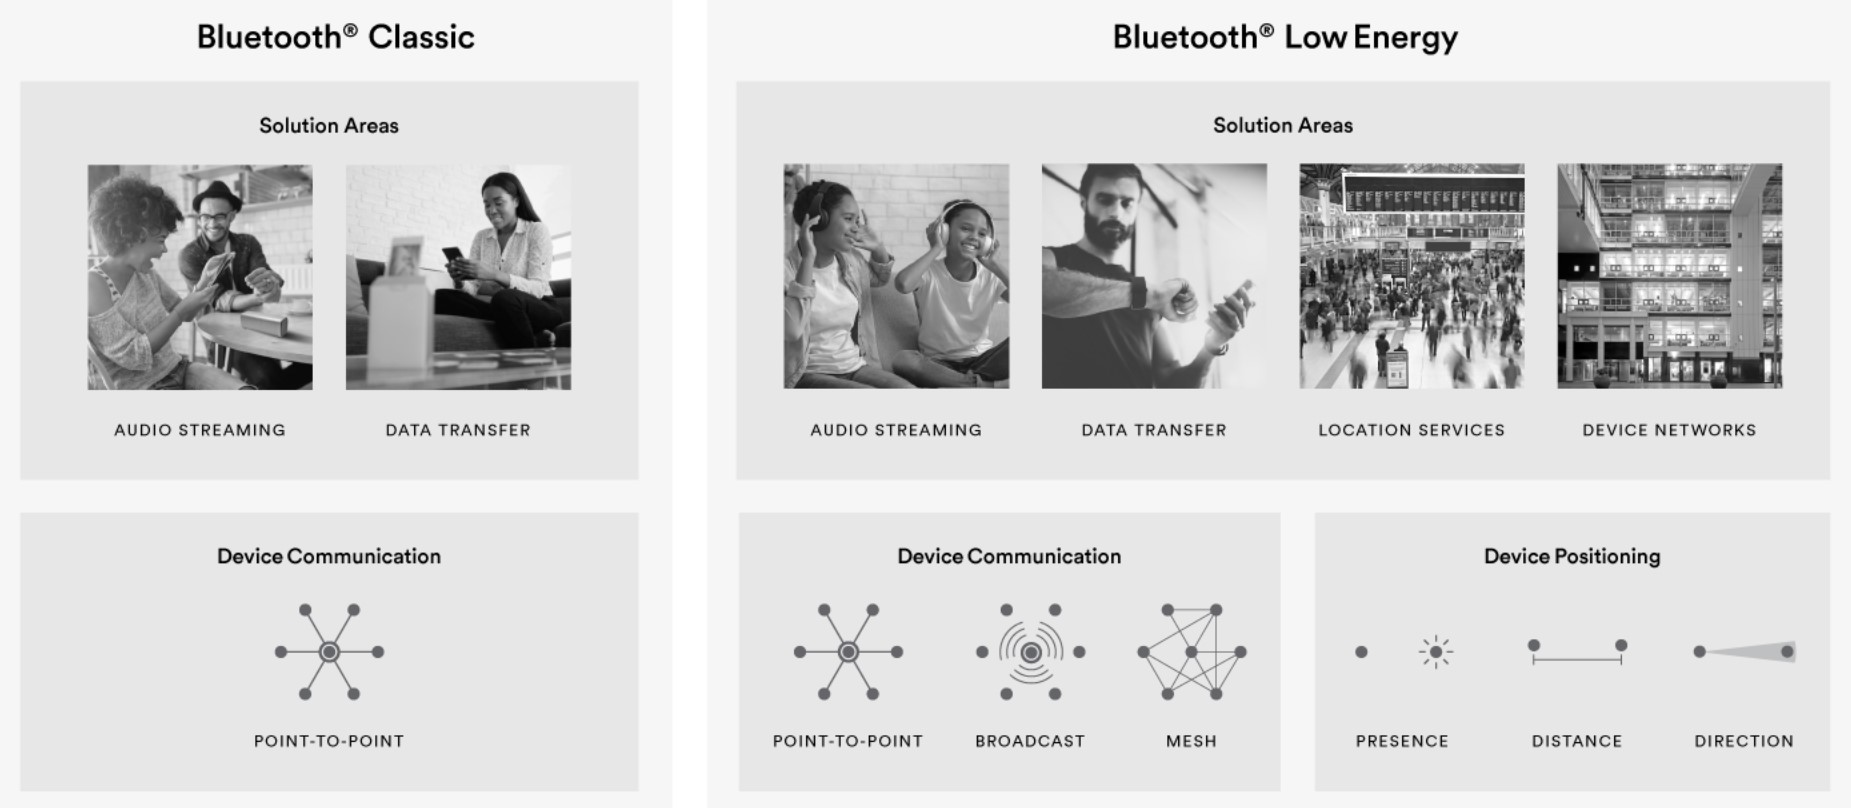
\includegraphics[width=\linewidth]{images/蓝牙}
    \end{figure}
\end{frame}


\begin{frame}[t]
    \frametitle{}
    \begin{block}{试一试：使用蓝牙功能分享一张图片给你的朋友}
        \begin{enumerate}
          \item 双方打开蓝牙
          \item 接收方：修改蓝牙名称为自己的名字
          \item 发送方：打开相册，选择一张照片，分享方式选择蓝牙
          \item 发送方：在蓝牙设备列表中找到你的朋友，发给他
          \item 接收方：收到蓝牙共享消息，选择“接受”
          \item 打开秒表，看看用蓝牙传输一张照片用时多久。
        \end{enumerate}
    \end{block}
\end{frame}


\begin{frame}
    \frametitle{蓝牙技术发展史}
    \begin{center}
        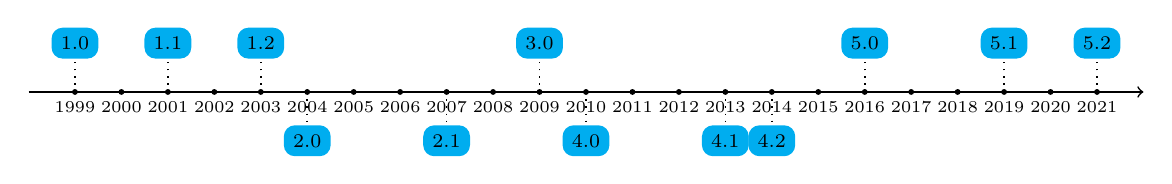
\begin{tikzpicture}[scale=0.59]
          \draw [->,semithick] (0,0) -- (24,0);
          \foreach \x [count=\i] in {1999,2000,2001,2002,2003,2004,2005,2006,2007,2008,2009,2010,2011,2012,2013,2014,2015,2016,2017,2018,2019,2020,2021}
          \filldraw ({\i},0) circle (.05) node [below,font=\fontsize{6}{6}\selectfont] {\x};
          \draw [dotted,semithick] (1,0) -- (1,0.7) node [above,rounded corners,rectangle,fill=cyan,font=\fontsize{7}{7}\selectfont] {1.0};
          \draw [dotted,semithick] (3,0) -- (3,0.7) node [above,rounded corners,rectangle,fill=cyan,font=\fontsize{7}{7}\selectfont] {1.1};
          \draw [dotted,semithick] (5,0) -- (5,0.7) node [above,rounded corners,rectangle,fill=cyan,font=\fontsize{7}{7}\selectfont] {1.2};
          \draw [dotted,semithick] (6,0) -- (6,-0.7) node [below,rounded corners,rectangle,fill=cyan,font=\fontsize{7}{7}\selectfont] {2.0};
          \draw [dotted,semithick] (9,0) -- (9,-0.7) node [below,rounded corners,rectangle,fill=cyan,font=\fontsize{7}{7}\selectfont] {2.1};
          \draw [dotted,semithick] (11,0) -- (11,0.7) node [above,rounded corners,rectangle,fill=cyan,font=\fontsize{7}{7}\selectfont] {3.0};
          \draw [dotted,semithick] (12,0) -- (12,-0.7) node [below,rounded corners,rectangle,fill=cyan,font=\fontsize{7}{7}\selectfont] {4.0};
          \draw [dotted,semithick] (15,0) -- (15,-0.7) node [below,rounded corners,rectangle,fill=cyan,font=\fontsize{7}{7}\selectfont] {4.1};
          \draw [dotted,semithick] (16,0) -- (16,-0.7) node [below,rounded corners,rectangle,fill=cyan,font=\fontsize{7}{7}\selectfont] {4.2};
          \draw [dotted,semithick] (18,0) -- (18,0.7) node [above,rounded corners,rectangle,fill=cyan,font=\fontsize{7}{7}\selectfont] {5.0};
          \draw [dotted,semithick] (21,0) -- (21,0.7) node [above,rounded corners,rectangle,fill=cyan,font=\fontsize{7}{7}\selectfont] {5.1};
          \draw [dotted,semithick] (23,0) -- (23,0.7) node [above,rounded corners,rectangle,fill=cyan,font=\fontsize{7}{7}\selectfont] {5.2};
      \end{tikzpicture}
      \end{center}
    \begin{table}
        \centering
        \begin{tabular}{cccc}
            \bottomrule
            蓝牙版本 & 最大传输速度 & 传输距离 &  \\ \hline
            蓝牙1 & 1\ Mbit/s & 10米 &  \\ 
            蓝牙2 & 3\ Mbit/s & 10米 &  \\ 
            蓝牙3 & 24\ Mbit/s & 10米 &  \\ 
            蓝牙4 & 48\ Mbit/s & 50米 &  \\ 
            蓝牙5 & 48\ Mbit/s & 300米 &  \\ \toprule
        \end{tabular}
    \end{table}
\end{frame}

% 蓝牙是一种短距离无线通信技术，它最初是为无线耳机设计的，但后来扩展到视频游戏控制器、打印机、扬声器等应用。目前有两种蓝牙版本，即经典蓝牙和蓝牙低功耗（BLE）。经典蓝牙（Bluetooth Classic）最初用于消费设备之间的点对点或点对多点（最多七个从属节点）的数据交换。后来，针对功耗进行优化，引入了蓝牙低功耗技术以此解决功耗敏感型的IoT应用需求。

% 支持BLE的IoT设备通常与智能设备（如智能手机）一起使用，在这里，智能手机主要负责向云端传输数据。现在，BLE被广泛集成到可穿戴设备（如智能手表、血糖仪、脉搏血氧仪等）以及智能家居设备（如门锁）中。

\begin{frame}
    \frametitle{蓝牙技术发展史}
    \begin{multicols}{2}
        \begin{enumerate}
          \item {\cbf{第一代蓝牙：短距离通讯早期探索}}
            \begin{itemize}
              \item {\bfseries 1.0} 从无到有
              \item {\bfseries 1.1} 列入 IEEE 802.15.1 标准
              \item {\bfseries 1.2} 改善抗干扰调频
            \end{itemize}
          \item {\cbf{第二代蓝牙：发力传输速率的时代}}
            \begin{itemize}
              \item {\bfseries 2.0} Enhanced Data Rate，3Mbps
              \item {\bfseries 2.1} 改善配对体验，支持NFC
            \end{itemize}
          \item {\cbf{第三代蓝牙：High Speed高速传输}}
            \begin{itemize}
              \item {\bfseries 3.0} 高速数据传输，达24Mbps 
            \end{itemize}
          \item {\cbf{第四代蓝牙：主推低功耗}}
            \begin{itemize}
              \item {\bfseries 4.0} BLE（Bluetooth Low Energy）
              \item {\bfseries 4.1} 支持与 LTE 无缝协作
              \item {\bfseries 4.2} 改善隐私保护
            \end{itemize}
          \item {\cbf{第五代蓝牙：开启物联网时代大门}}
            \begin{itemize}
              \item {\bfseries 5.0} 针对 IoT 物联网进行底层优化
              \item {\bfseries 5.1} 提高定位精度
              \item {\bfseries 5.2} LE功耗控制，LE同步信道
              \item {\bfseries 5.3} 提高LE通讯效率、降低功耗
            \end{itemize}
        \end{enumerate}
    \end{multicols}
\end{frame}


\begin{frame}[t]
    \frametitle{}
    \begin{question}
        蓝牙技术数据传输速度慢，容易受干扰，用户可能会遇到配对问题或连接蓝牙设备时遇到困难，连接设备数量有限……

        蓝牙缺点这么多，为什么还依然长盛不衰？
    \end{question}
\end{frame}


\begin{frame}
    \frametitle{$\vcenter{\hbox{
\includegraphics[height=14pt]{images/NearLinkB}}}$ NearLink 星闪 \link{http://sparklink.org.cn/news_info.php?id=669}}
    我们为何需要星闪？

    \begin{enumerate}
      \item 融合架构，一标多模
          \begin{itemize}
            \item SLB：对标Wi-Fi，应对高速率、大传输、高质量连接场景
            \item SLE：对标蓝牙，满足低功耗轻量级连接需求
          \end{itemize}
      \item 技术更先进、标准更领先、体验更突出
      \item 自主可控
    \end{enumerate}
    \begin{figure}[htpb]
      \centering
      
\includegraphics[width=\linewidth]{星闪优势}
    \end{figure}
\end{frame}


\begin{frame}
    \frametitle{$\vcenter{\hbox{
\includegraphics[height=14pt]{images/zigbee}}}$ Zigbee}
    \qquad Zigbee是一种新兴的低成本、低功耗的短距离无线通信协议，能够广泛的应用于军事、工业、智能家居等领域。但由于Zigbee技术出现较晚，其规范及应用仍在不断的完善和发展之中。

    \qquad Zigbee是基于IEEE802.15.4协议发展起来的一种短距离无线通信技术，功耗低，被业界认为是最有可能应用在工控场合的无线方式。ZigBee可工作在2.4GHz(全球流行)、868MHz(欧洲流行)和915 MHz(美国流行)3个频段上，分别具有最高250kbit/s、20kbit/s和40kbit/s的传输速率,它的传输距离在10-75m的范围内，但可以继续增加。
    \begin{multicols}{3}
        \begin{itemize}
          \item 低功耗
          \item 低成本
          \item 网络容量大
          \item 短时延
          \item 近距离
          \item 低速率
          \item 高安全
          \item 免执照频段
          \item 数据传输可靠
        \end{itemize}
    \end{multicols}
\end{frame}

\begin{frame}
  \frametitle{$\vcenter{\hbox{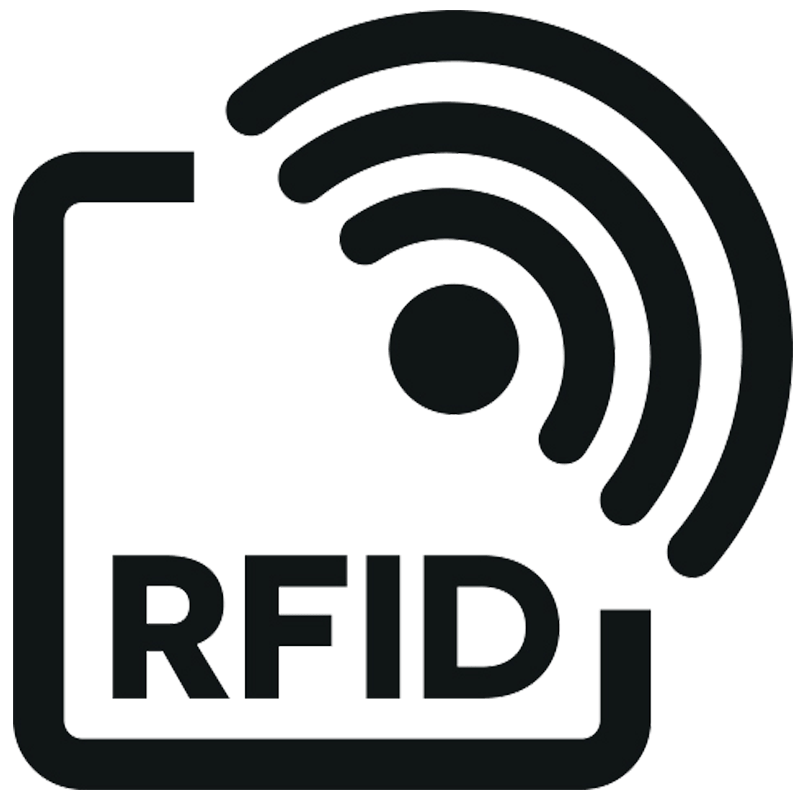
\includegraphics[height=14pt]{images/RFID}}}$ RFID 射频识别}
  射频识别（RFID）是一种无接触自动识别技术，利用射频信号在短距离内将少量数据从RFID标签传输到阅读器。RFID广泛应用于各种领域，从门禁控制到动物跟踪，从自动收费到供应链中的货物跟踪等。通过在各种产品和设备上贴上RFID标签，企业可以实时跟踪库存和资产，从而实现更好的库存和生产计划以及优化的供应链管理。

  \begin{figure}[htpb]
    \centering
    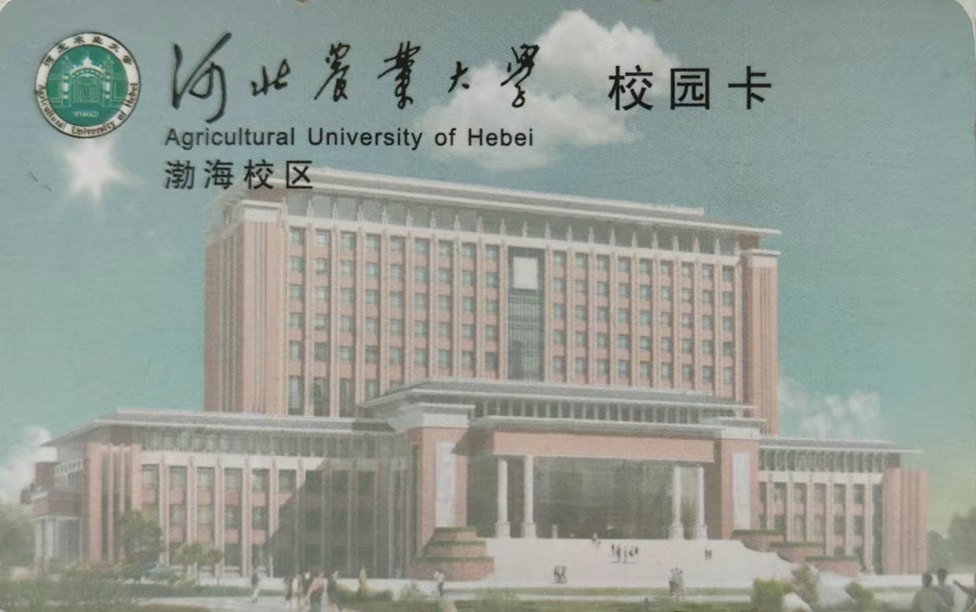
\includegraphics[width=.48\linewidth]{images/校园卡} \quad
    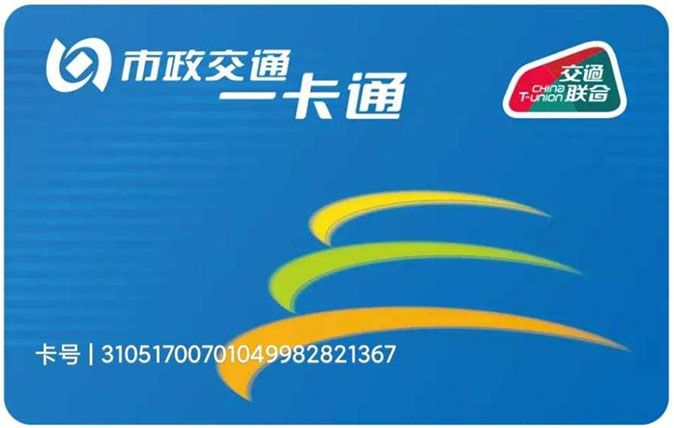
\includegraphics[width=.48\linewidth]{images/公交卡}
\end{figure}
\end{frame}

\begin{frame}
  \frametitle{RFID系统的组成}
  RFID应用系统一般由读写器、标签和计算机系统等部分组成，有些简易的RFID系统则只是由读写器与标签组成。

  读写器和标签可以构成一个简单的应用系统，复杂的应用需要一个读写器同时读取n个标签，更复杂的应用系统则需要由计算机系统参与读取数据。

% 射频标签物理上由三部分组成：标签（tag）、天线、读写器。
% 标签(Tag)：由耦合元件及芯片组成，每个标签有唯一的电子编码，高容量电子标签有用户写入区，附着在物体上标识目标对象；
% 读写器(Reader)：读取(有时还可以写入)标签信息的设备，可设计为手持式或固定式；
% 天线(Antenna)：在标签和读取器间传递射频信号。

  \begin{figure}[htpb]
    \centering
    
\includegraphics[width=\linewidth]{RFID组成}
  \end{figure}
\end{frame}

\begin{frame}
  \frametitle{RFID系统的基本工作原理}
  \begin{enumerate}
    \item 由阅读器通过发射天线发送特定频率的射频信号，当电子标签进入有效工作区域时产生感应电流，从而获得能量、电子标签被激活，使得电子标签将自身编码信息通过内置射频天线发送出去；
    \item 阅读器的接收天线接收到从标签发送来的调制信号，经天线调节器传送到阅读器信号处理模块，经解调和解码后将有效信息送至后台主机系统进行相关的处理；
  \end{enumerate}
    \begin{minipage}{0.38\linewidth}
          \begin{itemize}
            \item[3.]主机系统根据逻辑运算识别该标签的身份，针对不同的设定作出相应的处理和控制，最终发出指令信号控制阅读器完成相应的读写操作。
          \end{itemize}
      \end{minipage}\hfill
      \begin{minipage}{0.58\linewidth}
        \begin{figure}[htpb]
          \centering
          
\includegraphics[width=.9\linewidth]{RFID原理}
        \end{figure}
      \end{minipage}

\end{frame}

\begin{frame}
    \frametitle{RFID工作频率}
    \begin{itemize}
      \item \cbf{低频(LF)}
      
      30KHz – 300KHz, 典型的工作频率有125kHz、225kHz
      
      电子标签的成本较低、标签内保存的数据量较少、阅读距离较短(小于10cm)

      典型应用有：动物识别、容器识别、工具识别、门禁和安全管理系统。
      \item \cbf{高频(HF)}
      
      3MHz – 30MHz, 典型的工作频率有13.56MHz
      
      读取距离一般小于1米，数据传输速率较高
      \item \cbf{超高频(UHF)/微波}
      
      > 300MHz，典型的工作频段有915MHz、2.45GHz、5.8GHz

      电子标签及读写器成本较高、标签内保存的数据量较大、阅读距离较远（可达几米至十几米），适应物体高速运动性能好。

      典型应用包括：移动车辆识别、仓储物流管理和应用
    \end{itemize}
\end{frame}


\begin{frame}
    \frametitle{RFID技术在农业中的应用：智慧养殖}
    通过RFID技术对奶牛的身份信息进行识别，通过姿态传感器可以检测奶牛的行为，包括进食、排泄、分娩、休息。同时可有在牛的饲料装置下加入压力传感器，从而可以检测出奶牛的进食量。
    \begin{figure}[htpb]
        \centering
        
\includegraphics[height=.25\linewidth]{奶牛RFID}
        
\includegraphics[height=.25\linewidth]{奶牛传感器}
    \end{figure}
\end{frame}


\begin{frame}
    \frametitle{支付宝“碰一碰”支付\link{https://36kr.com/p/2855558959057794}}
    \begin{figure}[htpb]
        \centering
        
\includegraphics[width=\linewidth]{碰一碰}
    \end{figure}
\end{frame}


\begin{frame}
  \frametitle{$\vcenter{\hbox{
\includegraphics[height=13pt]{images/nfc}}}$ NFC 近场通信}
    \begin{minipage}{0.38\linewidth}
      NFC是在RFID基础上发展而来的，增加了点对点通信功能，可以快速建立蓝牙设备之间的P2P（点对点）无线通信。
      
      NFC可以理解为RFID技术的一个子集，使用的是13.56MHz频段。      
      \end{minipage}\hfill
      \begin{minipage}{0.58\linewidth}
        \begin{figure}[htpb]
          \centering
          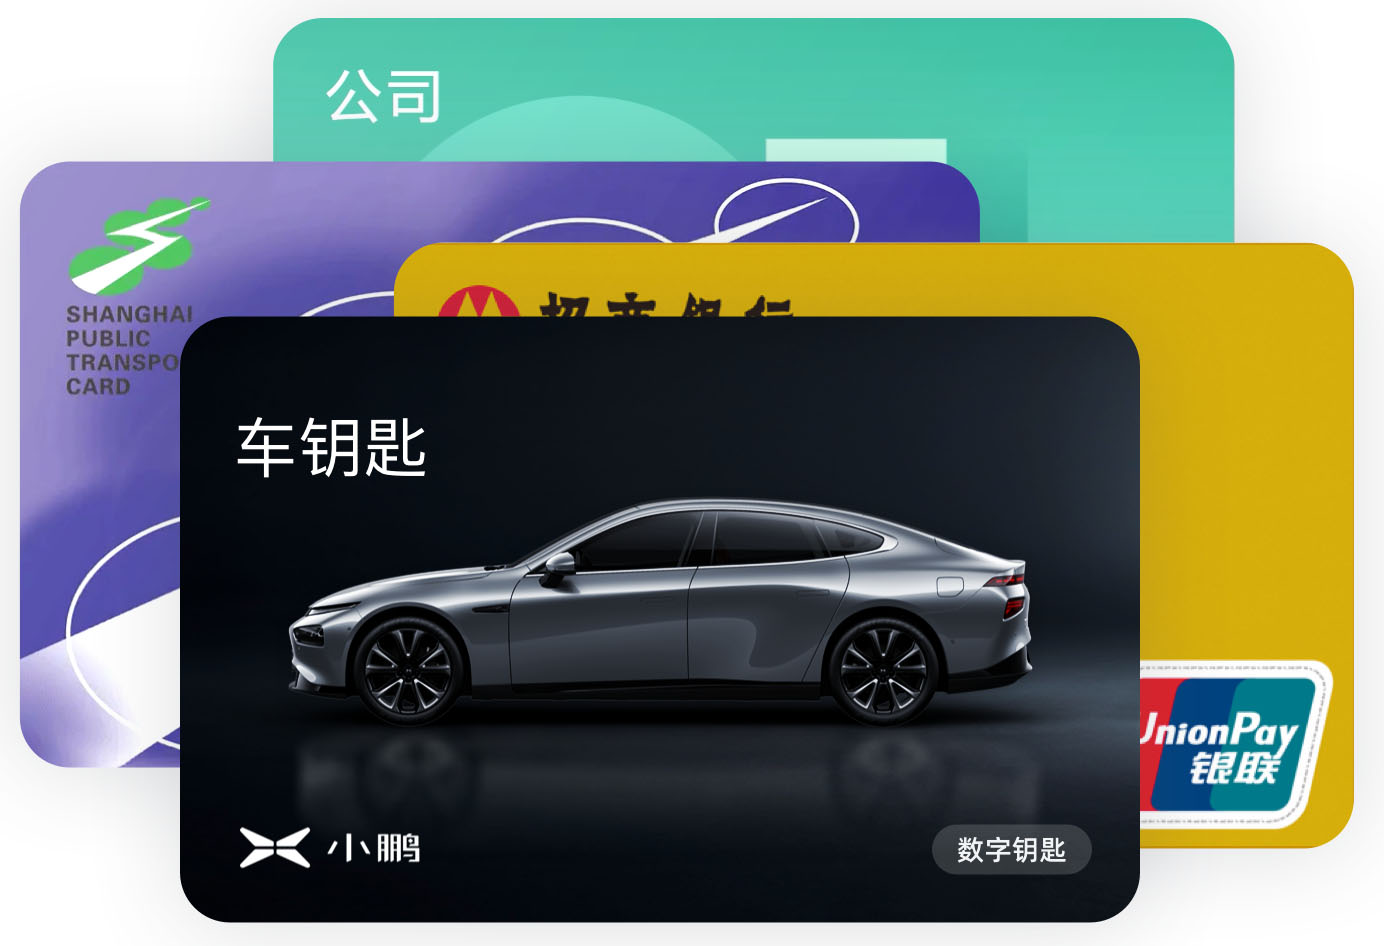
\includegraphics[width=\linewidth]{images/NFC卡}
        \end{figure}
      \end{minipage}
\end{frame}


\begin{frame}
    \frametitle{}
    \begin{block}{小调查：你最常用的手机支付方式是？}
        \begin{itemize}
          \item[A：] 支付宝
          \item[B：] 微信
          \item[C：] 其他
        \end{itemize}
    \end{block}
\end{frame}


\begin{frame}
    \frametitle{$\vcenter{\hbox{
\includegraphics[height=14pt]{images/UWB}}}$ UWB 超宽带通信}
    \emph{一些技术的真正实用价值，有时需要多年以后才能得到体现。}

    曾经UWB被认定会成为“短距离无线传输”领域的主流技术，但最终没有“卷”过WiFi和BLE蓝牙技术。在消费级市场领域遇冷10多年后，随着技术标准的不断完善，还有苹果等消费电子大厂加持，UWB重新回到了大家的视野中。
    \bigskip

      \begin{minipage}{0.48\linewidth}
            \begin{figure}[htpb]
              \centering
              {\bfseries 定位精度高}
              \smallskip

              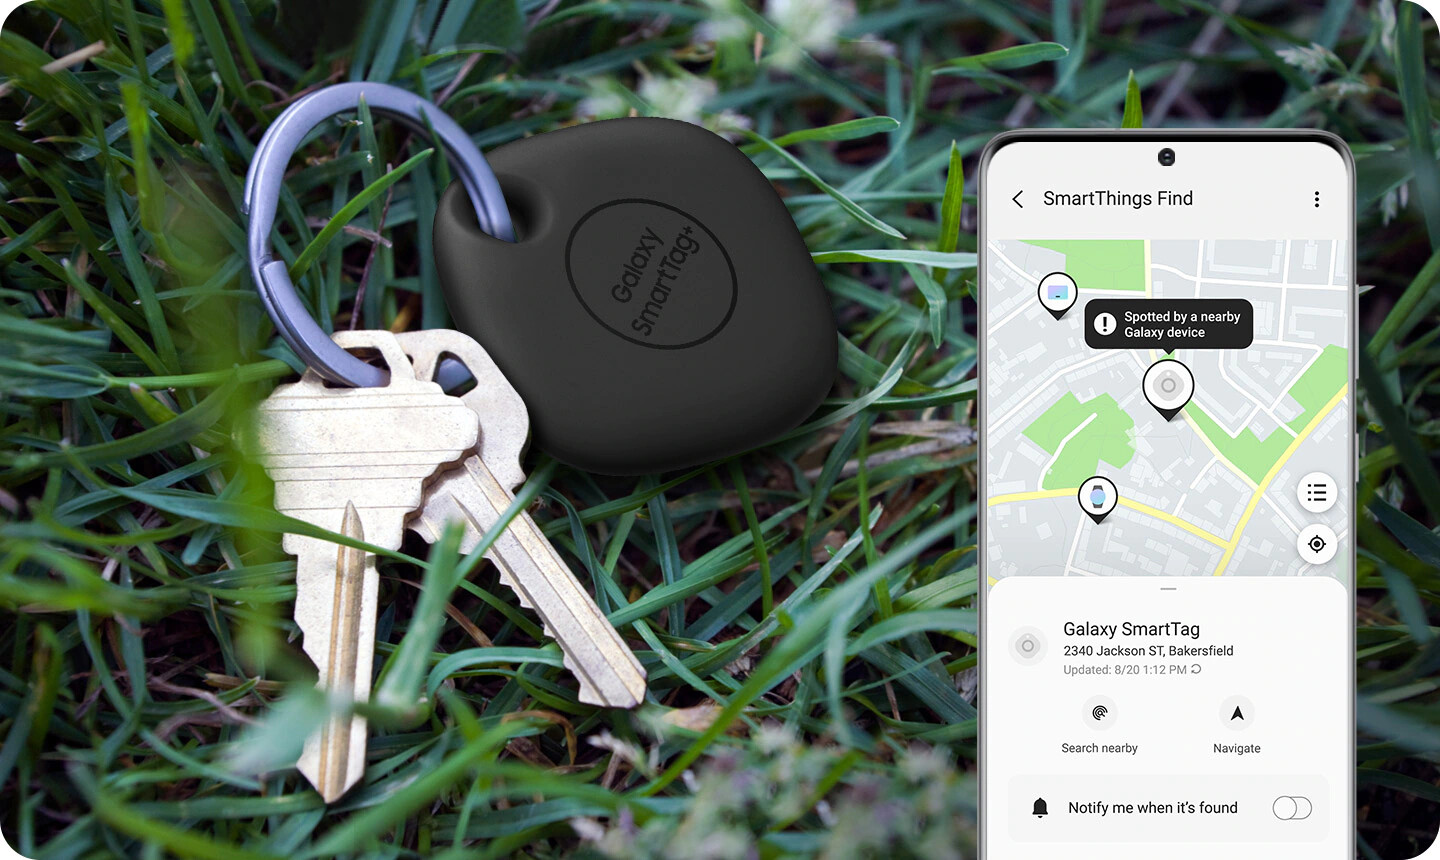
\includegraphics[height=.5\linewidth]{images/smarttag+}
            \end{figure}
        \end{minipage}\hfill
        \begin{minipage}{0.48\linewidth}
          \begin{figure}[htpb]
            \centering
            {\bfseries 传输速率高}
            \smallskip

            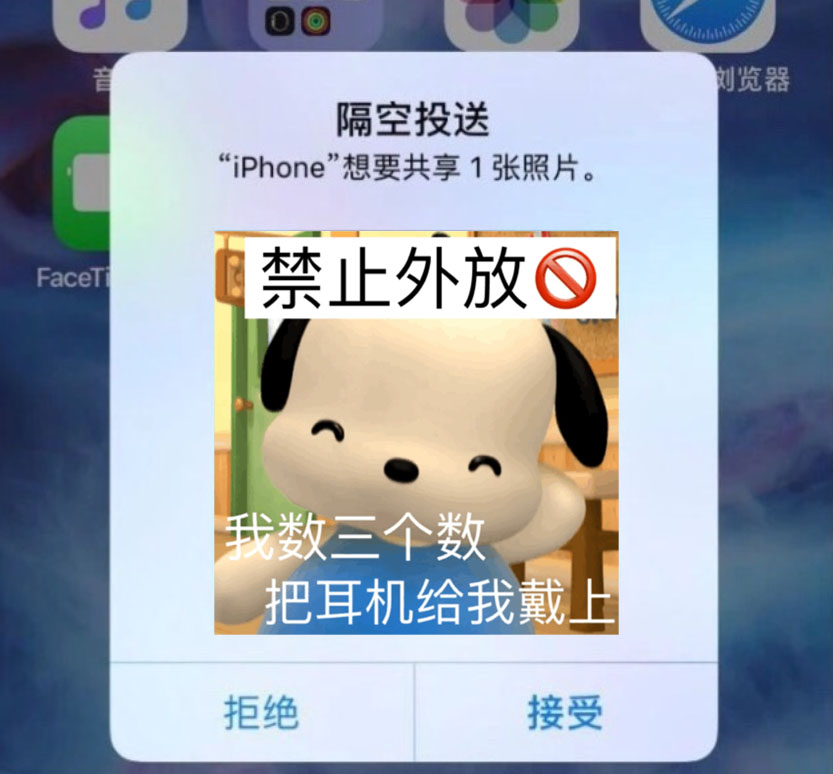
\includegraphics[height=.5\linewidth]{images/隔空投送}
          \end{figure}
        \end{minipage}
\end{frame}


\begin{frame}
    \frametitle{汽车数字钥匙}
    数字钥匙采用NFC、BLE（蓝牙）、UWB通信技术，将NFC智能卡、智能手机、智能手表和智能手环等智能终端设备变成车钥匙，从而实现无钥匙进入和启动、为他人远程钥匙授权、个性化的车辆设置等便捷功能。
    \begin{itemize}
      \item {\bfseries 第一代数字钥匙} \quad 基于NFC
      
      基本没有位置感知的能力。车主需要将数字钥匙贴近车身才能开启车门。
      \item {\bfseries 第二代数字钥匙} \quad NFC+BLE
      
      通信距离比第一代更远。可以通过蓝牙信号的强弱粗略感知车与钥匙的位置关系，但其感知精度与准确性都有所欠缺。
      \item {\bfseries 第三代数字钥匙} \quad NFC+BLE+UWB
      
      位置感知精度得到了质的飞跃。极大地提升了数字钥匙的安全性。
    \end{itemize}
\end{frame}

% https://zhuanlan.zhihu.com/p/458294241

% https://zhuanlan.zhihu.com/p/180082384

% 智能钥匙系统采用无线射频识别（RFID）技术，通常情况下，当车主走近车辆大约一米以内距离时，门锁就会自动打开并解除防盗；当离开车辆时，门锁会自动锁上并进入防盗状态。当车主进入车内时，车内检测系统会马上识别智能卡，这时只需轻轻按动启动按钮(或旋钮)，就可以正常启动车辆，整个过程，车钥匙无须拿出。

% 常规的无钥匙解锁的过程中，大概是这样的：钥匙会给车子发送一个信号，然后车子会和实体钥匙 or 手机钥匙发过来的信号进行确认，然后解锁车辆。

% 但是需要注意的是，大多数无钥匙进入系统只是通过信号强度来确定车辆驾驶员是否在范围内。也就是说，只要把这个沟通过程的信号放大，使得车子和钥匙「以为」车主就在附近，即可完成解锁操作。

% 这就产生了一种攻击方式：中继站攻击。比如说，我在家睡觉，钥匙就在旁边，靠近车辆的小偷会拉门把手假装开车门，然后通过手中的中继站收集来自车辆的请求解锁信号，这个信息会发送到靠近我身边钥匙的另外一个人的中继站里，而后发射到钥匙里，钥匙在收到信号后会返回一个有效信号，通过两个中继站回传到车内。中继站的作用就是放大了车子和钥匙沟通的信号强度，使得车子和钥匙「以为」车主就在车旁边，然后完成解锁动作，小偷就这样把车偷走了。

% UWB计算距离使用的原理是飞行时间（ToF），即发送端发射一个信号，接收端在收到这个信号之后经过协议定义的延迟后再发回给发送端，这样发送端只要比较发送和接受信号的时间差并乘以光速就能获得发送端与接收端之间的距离，从而可以实现亚米级别的距离精度。

% 通过这种高精度的定位，系统会通过钥匙到车子的信号传递时间来计算用户与车子的距离，如果窃贼想要通过中继站增强信号来获得开门权限，当系统探测到用户到车子的距离超出钥匙控车的最远距离，即会判定这是一次攻击，不会开启车门。

% 可以有效避免中继站攻击，对于追求安全的车厂们来说，很有吸引力，而且，当手机上拥有 UWB、蓝牙和 NFC 三个功能时，可以为用户提供更安全且精准的无钥匙进入体验：使用蓝牙唤醒 UWB，加密传输数据功能，UWB 则用于精准定位，而 NFC 则是用于手机没电情况下的备用进入手段。

\begin{frame}
    \frametitle{$\vcenter{\hbox{
\includegraphics[height=14pt]{images/nbiot}}}$ NB-IoT 窄带物联网}
    NB-IoT是基于蜂窝网络的窄带物联网。

    特点是广覆盖、大规模、低功耗、低成本。
    % 在4G技术定义初期，并没有把物联网的需求纳入考虑，因此业界后来又发展出NB-IoT，以补上这个缺口。 5G则与4G不同，在标准定义初期，就把物联网应用的需求纳入考虑，并制定出对应的mMTC技术标准。 不过，目前还很难断言mMTC是否会完全取代NB-IoT，因为mMTC与NB-IoT虽然在应用领域有所重迭，但mMTC会具备一些NB-IoT所没有的特性，反之亦然。 像是极低的网络等待时间，就是NB-IoT所没有的特性。

    \begin{figure}[htpb]
      \centering
      
\includegraphics[width=.8\linewidth]{NB-IOT}
    \end{figure}
\end{frame}

\begin{frame}
  \frametitle{mMTC}
  mMTC 是 5G 应用最为广泛的三大重要场景之一，专为物联网而生。
    \begin{minipage}{0.38\linewidth}
          \begin{center}
            \bf{5G三大应用场景：}
            \bigskip

              \begin{tikzpicture}
                \draw [rounded corners,fill=LightCyan1] (0,0) rectangle (5,1) node [midway] {mMTC 海量物联网通信};
                \draw [rounded corners,fill=LightCyan1,shift={(0,1.2)}] (0,0) rectangle (5,1) node [midway] {uRLLC 高可靠低时延通信};
                \draw [rounded corners,fill=LightCyan1,shift={(0,2.4)}] (0,0) rectangle (5,1) node [midway] {eMBB 增强移动宽带};
              \end{tikzpicture}
          \end{center}
      \end{minipage}\hfill
      \begin{minipage}{0.58\linewidth}
        \vspace{1em}
        \begin{itemize}
          \item 一平方公里内，能够承载100万个终端；
          \item 最差的信号环境下，时延小于10s；
          \item 最差信号环境下，电池寿命大于十年。
        \end{itemize}
        \begin{figure}[htpb]
          \centering
          
\includegraphics[width=.7\linewidth]{智慧城市}
        \end{figure}
      \end{minipage}
\end{frame}

%   5G的三大业务场景eMBB、URLLC、mMTC：

%  eMBB：英文全称Enhanced Mobile Broadband，即增强移动宽带，是利用5G更好的网络覆盖及更高的传输速率来为用户提供更好的上网接入服务，使得无线上网具有更高的上网速率和更稳定的传输，给客户带来的最直观的感受就是网速的大幅提升，即便是观看 4K 高清视频，峰值能够达到 10Gbps。

%  URLLC：英文全称Ultra Reliable & LowLatency Communication，即低时延高可靠，如名称所述，URLLC有两个基本特点，即高可靠和低时延，可以广泛应用于如AR/VR、工业控制系统、交通和运输（如无人驾驶）、智能电网和智能家居的管理、交互式的远程医疗诊断等。

%  mMTC：英文全称Massive Machine Type Communication，即海量物联网通信或大规模物联网业务，5G 低功耗、大连接和低时延高可靠的特性很好地适应了面向物联网的业务，可以重点解决传统移动通信无法很好支持地物联网及垂直行业应用。低功耗大连接场景主要面向智慧城市、环境监测、智能农业、森林防火等以传感和数据采集为目标的应用场景，具有小数据包、低功耗、海量连接等特点。这类终端分布范围广、数量众多，不仅要求网络具备超千亿连接的支持能力，满足 100 万 /km2 连接数密度指标要求，而且还要保证终端的超低功耗和超低成本。

\begin{frame}
    \frametitle{$\vcenter{\hbox{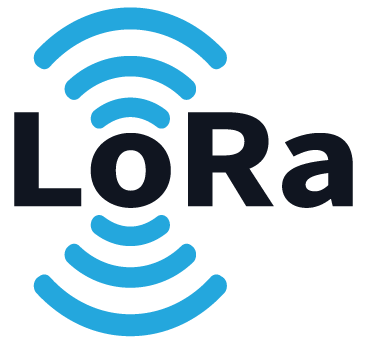
\includegraphics[height=14pt]{images/lora}}}$ Lora}
      \begin{minipage}{0.32\linewidth}
        \bf{物联网的无线通信技术：}
        \begin{itemize}
          \item 短距离通信技术
            \begin{itemize}
              \item WiFi
              \item 蓝牙
              \item Zigbee等
            \end{itemize}
          \item 广域网通信技术
            \begin{itemize}
              \item NB-IoT
              \item LoRa
            \end{itemize}
        \end{itemize}
      \end{minipage}\hfill
      \begin{minipage}{0.65\linewidth}
        LoRa和NB-IoT的技术特点非常相似，都是低功耗、广覆盖，适合海量连接场景。其最主要的不同就是，NB-IoT是运营商建网和提供服务，而LoRa是自建网络。

        \begin{itemize}
          \item[\bf{优势}] 自组网络。企业可以自主运营，可以把运营数据掌握在自己手中；自主把控网络质量，根据业务需要扩展网络，对网络覆盖可快速优化补充。
          \item[\bf{风险}] LoRa技术中，LoRa芯片处在整个产业链中处于基础核心地位，目前美国Semtech公司是LoRa芯片的核心供应商，掌握着LoRa底层技术的核心专利。
        \end{itemize}
      \end{minipage}
\end{frame}

\begin{frame}
    \frametitle{无线通信技术对比}
\begin{table}[]
    \begin{tabular}{@{}cll@{}}
    \toprule
           & \multicolumn{1}{c}{优点} & \multicolumn{1}{c}{缺点} \\ \midrule
    蓝牙     & 功耗低，便宜，延时低             & 容易受到信号干扰，联网耗时较久        \\
    WiFi   & 传输速率高                  & 信号覆盖范围有限，功耗大           \\
    Zigbee & 容量大，安全性高，功耗低           & 传输距离短，传输速率受限           \\
    Lora   & 传输距离远，穿透障碍物能力较强        & 速率低，传输时延较大             \\
    NB-IoT & 覆盖超强，海量接入，低功耗，低成本      & 速率较低，成本高               \\
    4G     & 传输速度更快，网络延迟更低          & 成本高，更高的能源消耗            \\ \bottomrule
    \end{tabular}
    \end{table}
\end{frame}

\begin{frame}
    \frametitle{如何选择最适合的物联网无线技术？}
    物联网应用中有许多优秀的无线通信技术。然而，没有一种技术是面面俱到的。要选择合适的物联网无线技术，需要根据具体需求来评估，在功耗、数据范围和带宽之间进行权衡，同时还要考虑电池大小、成本、传输距离以及固件更新等因素。
    \begin{itemize}
      \item 您需要传输多少数据？
      \item 需要的功率是多少？
      \item 数据源离互联网有多远？
      \item 服务费用有多高？
      \item 这些设备将在哪里使用？
    \end{itemize}
\end{frame}


\begin{frame}[t]
    \frametitle{}
    \begin{block}{选择任一话题进行思考讨论}
        \begin{enumerate}
          \item 探讨物联网技术的应用
          \item 同学们接触过哪些物联网设备？它使用了什么技术？
          \item 你认为物联网技术在农业中可以起到什么作用？
          \item 为什么物联网无线接入技术对农业物联网的应用非常关键？
          \item 为什么NFC这样一个看起来、用起来都要比二维码更好的技术始终未能得到普及？
          \item 你认为未来的移动支付会是什么样子的？
          \item 微信圆形的小程序码，属于QR码吗？
        \end{enumerate}
    \end{block}
\end{frame}
